% Pham vi goc: Muc 5.4 - Mien tin cay va so sanh dong thoi.
% File nay chi chia khuc noi dung, chua gan ten thanh vien phu trach.
\section{Miền tin cậy và so sánh đồng thời}
\sectionframe{Miền tin cậy và so sánh đồng thời}

\begin{frame}{Miền tin cậy và so sánh đồng thời}
  \begin{block}{Phạm vi nội dung}
    Chuyển từ kiểm định một điểm \(\boldsymbol{\mu}_0\) sang tập các giá trị \(\boldsymbol{\mu}\) còn hợp lý với dữ liệu.
  \end{block}
  \begin{itemize}
    \item Miền tin cậy đồng thời cho vectơ trung bình.
    \item So sánh đồng thời các trung bình thành phần.
    \item Cách diễn giải miền ellipsoid hoặc khoảng tin cậy Bonferroni.
  \end{itemize}
\end{frame}
% =====================================================================
% PHẦN NỘI DUNG: NGUYỄN MINH ĐỨC
% =====================================================================

% Mục 5.4 - Phần 3: Phương pháp so sánh bội Bonferroni và phần kết
\begin{frame}{Động cơ: khi chỉ quan tâm các trung bình thành phần}
  \begin{itemize}
    \item Khoảng $T^2$ quá rộng nếu chỉ áp dụng cho riêng $p$ trung bình thành phần.
    \item Xét Hình 5.2: nếu $\mu_1$ nằm trong khoảng $T^2$ của nó và $\mu_2$ nằm trong khoảng $T^2$ của nó thì $(\mu_1,\mu_2)$ nằm trong hình chữ nhật tạo bởi hai khoảng này.
    \item Hình chữ nhật này \textbf{chứa elip tin cậy và còn hơn thế nữa}: xác suất phủ đồng thời $\mu_1,\mu_2$ lớn hơn $0{,}95$.
    \item Thông thường, ta chỉ quan tâm một \textbf{số nhỏ} $m$ phát biểu tin cậy $\Rightarrow$ có thể xây dựng khoảng đồng thời \textbf{ngắn hơn (chính xác hơn)} khoảng $T^2$.
    \item Cách làm này gọi là \textbf{phương pháp Bonferroni}, vì xuất phát từ một bất đẳng thức xác suất cùng tên.
  \end{itemize}
  \note{Câu hỏi có thể gặp: \emph{Vì sao $T^2$ quá rộng?} Vì khoảng $T^2$ đảm bảo cho mọi $\mathbf{a}$, còn ta chỉ cần $p$ trung bình. Hình chữ nhật tạo bởi các khoảng $T^2$ chứa elip tin cậy (elip có xác suất phủ đúng $0{,}95$) nên xác suất phủ của hình chữ nhật lớn hơn $0{,}95$, tức là ``dư'' độ tin cậy so với mức cần.}
\end{frame}
 
% ---------------------------------------------------------------------
\begin{frame}{Thiết lập bài toán}
  \begin{itemize}
    \item \textbf{Trước khi thu thập dữ liệu}, giả sử cần các phát biểu tin cậy về $m$ tổ hợp tuyến tính:
    \[
      \mathbf{a}_1'\boldsymbol{\mu},\; \mathbf{a}_2'\boldsymbol{\mu},\; \ldots,\; \mathbf{a}_m'\boldsymbol{\mu},
      \qquad \mathbf{a}'\boldsymbol{\mu} = a_1\mu_1 + a_2\mu_2 + \cdots + a_p\mu_p
    \]
    \item Gọi $C_i$ là phát biểu tin cậy về giá trị của $\mathbf{a}_i'\boldsymbol{\mu}$, với
    \[
      P[C_i \text{ đúng}] = 1-\alpha_i, \qquad i = 1,2,\ldots,m
    \]
    \item Mục tiêu: kiểm soát xác suất để \textbf{tất cả} $C_i$ cùng đúng.
  \end{itemize}
  \note{Câu hỏi có thể gặp: \emph{Vì sao phải chọn phát biểu trước khi thu thập dữ liệu?} Sách đặt giả thiết ``prior to the collection of data'' khi xây dựng phương pháp. Ngược lại, các khoảng $T^2$ ``lý tưởng cho dò quét dữ liệu'' vì hệ số tin cậy $1-\alpha$ không đổi với mọi cách chọn $\mathbf{a}$ (sách trang 226).}
\end{frame}
 
% ---------------------------------------------------------------------
\begin{frame}{Bất đẳng thức Bonferroni }
  \small
  \setlength{\abovedisplayskip}{2pt}
  \setlength{\belowdisplayskip}{2pt}
  \begin{align*}
    P[\text{tất cả } C_i \text{ đúng}] &= 1 - P[\text{ít nhất một } C_i \text{ sai}] \\
    &\ge 1 - \sum_{i=1}^m P(C_i \text{ sai}) = 1 - \sum_{i=1}^m \bigl(1 - P(C_i \text{ đúng})\bigr) \\
    &= 1 - (\alpha_1 + \alpha_2 + \cdots + \alpha_m) \tag{5-28}
  \end{align*}
  \footnotesize
  \begin{itemize}
    \item Cho phép kiểm soát \textbf{tỷ lệ sai số tổng thể} $\alpha_1+\cdots+\alpha_m$, \textbf{bất kể cấu trúc tương quan} đằng sau các phát biểu.
    \item Có thể kiểm soát tỷ lệ sai số cho một nhóm phát biểu quan trọng, và cân bằng bằng một lựa chọn khác cho các phát biểu ít quan trọng hơn.
  \end{itemize}
  \note{Câu hỏi có thể gặp: \emph{Bước dấu $\ge$ từ đâu?} Biến cố ``ít nhất một $C_i$ sai'' là hợp của các biến cố ``$C_i$ sai'', và xác suất của một hợp không vượt quá tổng các xác suất, nên $P[\text{ít nhất một sai}] \le \sum P(C_i \text{ sai})$; trừ hai vế từ $1$ ta được dấu $\ge$. Vì chỉ dùng tổng xác suất nên không cần biết các $C_i$ độc lập hay tương quan. Bước tiếp theo dùng $P(C_i \text{ sai}) = 1 - P(C_i \text{ đúng}) = \alpha_i$.}
\end{frame}
 
% ---------------------------------------------------------------------
\begin{frame}{Khoảng Bonferroni cho các trung bình thành phần}
  \begin{itemize}
    \item Không có thông tin về tầm quan trọng tương đối của các thành phần $\mu_i$ $\Rightarrow$ xét các khoảng $t$ riêng lẻ với $\alpha_i = \alpha/m$:
    \[
      \bar{x}_i \pm t_{n-1}\!\left(\frac{\alpha_i}{2}\right)\sqrt{\frac{s_{ii}}{n}}, \quad i=1,\ldots,m
    \]
    \item Vì $P\!\left[\bar{X}_i \pm t_{n-1}\!\left(\frac{\alpha}{2m}\right)\sqrt{\frac{S_{ii}}{n}} \text{ chứa } \mu_i\right] = 1-\frac{\alpha}{m}$, từ (5-28):
    \[
      P\!\left[\bar{X}_i \pm t_{n-1}\!\left(\tfrac{\alpha}{2m}\right)\sqrt{\tfrac{S_{ii}}{n}} \text{ chứa } \mu_i,\ \forall i\right]
      \ge 1 - \underbrace{\left(\tfrac{\alpha}{m}+\tfrac{\alpha}{m}+\cdots+\tfrac{\alpha}{m}\right)}_{m \text{ số hạng}} = 1-\alpha
    \]
  \end{itemize}
  \note{Câu hỏi có thể gặp: \emph{Vì sao là $t_{n-1}(\alpha/2m)$?} Khoảng $t$ hai phía có mức ý nghĩa $\alpha_i=\alpha/m$ dùng điểm phần trăm trên $100(\alpha_i/2)$ của phân phối $t$ với $n-1$ bậc tự do, tức $t_{n-1}\!\left(\frac{\alpha}{2m}\right)$ (cách định nghĩa $t_{n-1}(\alpha/2)$ ở trang 224). \emph{Vì sao chọn $\alpha_i=\alpha/m$?} Vì không biết thành phần nào quan trọng hơn, và $m$ số hạng $\alpha/m$ cộng lại đúng bằng $\alpha$.}
\end{frame}
 
% ---------------------------------------------------------------------
\begin{frame}{Khoảng Bonferroni và so sánh với khoảng $T^2$}
  Với mức tin cậy tổng thể $\ge 1-\alpha$, ta đưa ra $m=p$ phát biểu:
  \begin{equation*}
    \bar{x}_i - t_{n-1}\!\left(\frac{\alpha}{2p}\right)\sqrt{\frac{s_{ii}}{n}} \;\le\; \mu_i \;\le\; \bar{x}_i + t_{n-1}\!\left(\frac{\alpha}{2p}\right)\sqrt{\frac{s_{ii}}{n}}, \quad i=1,\dots,p \tag{5-29}
  \end{equation*}
  \begin{block}{So sánh (5-29) với (5-24)}
    Giá trị $t_{n-1}\!\left(\dfrac{\alpha}{2p}\right)$ thay cho $\sqrt{\dfrac{(n-1)\,p}{n-p}F_{p,n-p}(\alpha)}$; ngoài điểm thay thế này, các khoảng có \textbf{cùng cấu trúc}.
  \end{block}
  \note{Câu hỏi có thể gặp: \emph{Khác biệt duy nhất giữa hai phương pháp?} Chỉ ở hệ số nhân của $\sqrt{s_{ii}/n}$: $T^2$ dùng $\sqrt{p(n-1)F_{p,n-p}(\alpha)/(n-p)}$, Bonferroni dùng $t_{n-1}(\alpha/2p)$. Hai hệ số này được so sánh bằng số ở Bảng 5.4 (slide sau).}
\end{frame}
 
% ---------------------------------------------------------------------
\begin{frame}{Ví dụ 5.6: Khoảng Bonferroni 95\% (dữ liệu bức xạ lò vi sóng)}
  Dữ liệu ở Ví dụ 5.3 và 5.4: $n=42$, $p=2$, $\alpha_i = 0{,}05/2$, $i=1,2$.
  \[
    t_{41}\!\left(\frac{0{,}05}{2(2)}\right) = t_{41}(0{,}0125) = 2{,}327
  \]
  \begin{exampleblock}{Kết quả (hệ số $\sqrt{s_{ii}/n}$ lấy từ Ví dụ 5.3)}
    \begin{align*}
      \bar{x}_1 \pm t_{41}(0{,}0125)\sqrt{\tfrac{s_{11}}{n}} &= 0{,}564 \pm 2{,}327\sqrt{\tfrac{0{,}0144}{42}} \quad\text{hay}\quad 0{,}521 \le \mu_1 \le 0{,}607 \\[1ex]
      \bar{x}_2 \pm t_{41}(0{,}0125)\sqrt{\tfrac{s_{22}}{n}} &= 0{,}603 \pm 2{,}327\sqrt{\tfrac{0{,}0146}{42}} \quad\text{hay}\quad 0{,}560 \le \mu_2 \le 0{,}646
    \end{align*}
  \end{exampleblock}
  So với các khoảng $T^2$ ở Ví dụ 5.4: $(0{,}516;\,0{,}612)$ và $(0{,}555;\,0{,}651)$.
  \note{Câu hỏi có thể gặp: \emph{Giá trị $2{,}327$ từ đâu?} $m=p=2$ nên $\alpha/2m = 0{,}05/4 = 0{,}0125$; tra $t$ với $n-1=41$ bậc tự do ta được $t_{41}(0{,}0125)=2{,}327$ (theo sách). Các số $\bar{x}_1=0{,}564$, $\bar{x}_2=0{,}603$, $s_{11}=0{,}0144$, $s_{22}=0{,}0146$ lấy từ Ví dụ 5.3.}
\end{frame}
 
% ---------------------------------------------------------------------
\begin{frame}{Hình 5.4: Khoảng Bonferroni và khoảng $T^2$}
  \begin{columns}[T]
    \begin{column}{0.52\textwidth}
      \centering
      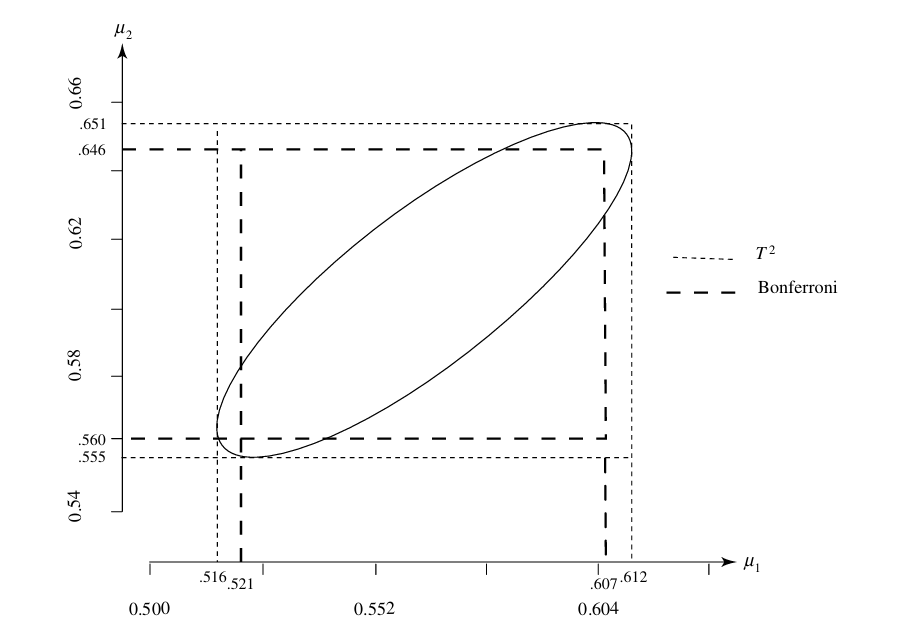
\includegraphics[width=\textwidth]{figures/figure_5_4.png}
    \end{column}
    \begin{column}{0.48\textwidth}
      \small
      \begin{itemize}
        \item Với mỗi trung bình thành phần, khoảng Bonferroni nằm \textbf{trong} khoảng $T^2$.
        \item Do đó hình chữ nhật tạo bởi hai khoảng Bonferroni nằm trong hình chữ nhật tạo bởi hai khoảng $T^2$.
        \item Nếu chỉ quan tâm các trung bình thành phần: Bonferroni cho ước lượng \textbf{chính xác hơn}.
        \item Miền tin cậy 95\% đối với $\boldsymbol{\mu}$ cho các giá trị hợp lý của cặp $(\mu_1,\mu_2)$ khi \textbf{tính đến tương quan} giữa các biến đo.
      \end{itemize}
    \end{column}
  \end{columns}
  \note{Chú ý: chú thích trong hình, đường chấm là khoảng $T^2$ (.516--.612; .555--.651), đường đứt nét là khoảng Bonferroni (.521--.607; .560--.646).}
\end{frame}
 
% ---------------------------------------------------------------------
\begin{frame}{So sánh độ dài: Bonferroni và $T^2$}
  \small
  \setlength{\abovedisplayskip}{2pt}
  \setlength{\belowdisplayskip}{2pt}
  Hai loại khoảng đều có dạng $\mathbf{a}'\bar{\mathbf{X}} \pm (\text{giá trị tới hạn})\sqrt{\mathbf{a}'\mathbf{S}\mathbf{a}/n}$. Khi $\alpha_i=\alpha/m$:
  \begin{equation*}
    \frac{\text{Độ dài khoảng Bonferroni}}{\text{Độ dài khoảng } T^2}
    = \frac{t_{n-1}(\alpha/2m)}{\sqrt{\dfrac{p(n-1)}{n-p}F_{p,n-p}(\alpha)}} \tag{5-30}
  \end{equation*}
  \vspace{-0.2cm}
  \begin{columns}[T]
    \begin{column}{0.46\textwidth}
      \footnotesize
      \begin{itemize}
        \item Tỷ số \textbf{không phụ thuộc} $\bar{\mathbf{X}}$ và $\mathbf{S}$.
        \item Với số nhỏ $m$ hàm $\mathbf{a}'\boldsymbol{\mu}$ chỉ định trước, khoảng Bonferroni luôn ngắn hơn; Bảng 5.4 cho thấy ngắn hơn bao nhiêu khi $m=p$.
      \end{itemize}
    \end{column}
    \begin{column}{0.52\textwidth}
      \centering
      {\scriptsize \textbf{Bảng 5.4} (Độ dài Bonferroni)/(Độ dài $T^2$), $1-\alpha=0{,}95$, $\alpha_i=0{,}05/m$\par}
      \vspace{2pt}
      \scriptsize
      \begin{tabular}{c|ccc}
        \toprule
        & \multicolumn{3}{c}{$m=p$} \\
        $n$ & 2 & 4 & 10 \\
        \midrule
        15       & 0,88 & 0,69 & 0,29 \\
        25       & 0,90 & 0,75 & 0,48 \\
        50       & 0,91 & 0,78 & 0,58 \\
        100      & 0,91 & 0,80 & 0,62 \\
        $\infty$ & 0,91 & 0,81 & 0,66 \\
        \bottomrule
      \end{tabular}
    \end{column}
  \end{columns}
  \note{Câu hỏi có thể gặp: \emph{Vì sao tỷ số không phụ thuộc $\bar{\mathbf{X}}$ và $\mathbf{S}$?} Hai loại khoảng có cùng dạng $\mathbf{a}'\bar{\mathbf{X}} \pm (\text{tới hạn})\sqrt{\mathbf{a}'\mathbf{S}\mathbf{a}/n}$, nên khi lập tỷ số độ dài, phần $\sqrt{\mathbf{a}'\mathbf{S}\mathbf{a}/n}$ triệt tiêu, chỉ còn tỷ số hai giá trị tới hạn. \emph{Đọc bảng thế nào?} Số $0{,}69$ ở $n=15$, $p=4$ nghĩa là khoảng Bonferroni chỉ dài bằng $69\%$ khoảng $T^2$.}
\end{frame}
 
% ---------------------------------------------------------------------
\begin{frame}{Khi nào dùng Bonferroni?}
  \begin{columns}[T]
    \begin{column}{0.48\textwidth}
      \begin{block}{Ưu điểm}
        \small
        \begin{itemize}
          \item Kiểm soát tỷ lệ sai số tổng thể $\alpha_1+\cdots+\alpha_m$, \textbf{bất kể cấu trúc tương quan}.
          \item Linh hoạt chia $\alpha_i$: nhóm phát biểu quan trọng dùng $\alpha_i$ khác với nhóm ít quan trọng.
          \item Với $m$ nhỏ, khoảng \textbf{ngắn hơn (chính xác hơn)} khoảng $T^2$ (Bảng 5.4).
          \item Dễ áp dụng, chỉ cần giá trị $t$.
        \end{itemize}
      \end{block}
    \end{column}
    \begin{column}{0.48\textwidth}
      \begin{block}{Phạm vi áp dụng}
        \small
        \begin{itemize}
          \item Chú ý đến một \textbf{số nhỏ} $m$ phát biểu tin cậy.
          \item Các phát biểu được \textbf{chỉ định trước khi thu thập dữ liệu}.
          \item Nếu muốn chọn $\mathbf{a}$ sau khi xem dữ liệu (dò quét dữ liệu), khoảng $T^2$ là lý tưởng vì $1-\alpha$ không đổi với mọi $\mathbf{a}$.
          \item Cho khoảng từng thành phần; để xét cặp $(\mu_i,\mu_k)$ có tính đến tương quan thì dùng elip tin cậy.
        \end{itemize}
      \end{block}
    \end{column}
  \end{columns}
  \note{Mọi ý trên đều có trong sách: ưu điểm ở trang 232 (bất đẳng thức 5-28 và hai nhận xét sau nó) và trang 234 (Bảng 5.4); phạm vi áp dụng ở trang 232 (``small number'', ``prior to the collection of data''), trang 226 (dò quét dữ liệu, elip 5-26) và trang 234 (miền tin cậy tính đến tương quan).}
\end{frame}
 
% ---------------------------------------------------------------------
\begin{frame}{Kết luận }
  \begin{itemize}
    \item Phương pháp Bonferroni cho khoảng \textbf{ngắn hơn} khi $m=p$ (Bảng 5.4).
    \item Vì \textbf{dễ áp dụng} và cho các khoảng tin cậy \textbf{tương đối ngắn} cần thiết cho suy diễn thống kê, ta thường áp dụng các \textbf{khoảng $t$ đồng thời dựa trên phương pháp Bonferroni}.
    \item Nếu cần các giá trị hợp lý cho cặp $(\mu_1,\mu_2)$ có tính đến tương quan giữa các biến, dùng \textbf{miền tin cậy} (elip) cho $\boldsymbol{\mu}$.
  \end{itemize}
  \note{Hai ý đầu là câu kết của mục 5.4 (trang 234). Ý thứ ba lấy từ cuối Ví dụ 5.6 (trang 233--234).}
\end{frame}